\section{Numerical Methods}\label{sec:numerical_methods}

In this section we will be looking at the numerical methods used to solve the PDE's given in the previous section. 

A time-dependent partial differential equation is first discretized in space, resulting in a semi-discrete system of ordinary differential equations (or differential-algebraic equations). The spatial discretization may be performed using methods such as the Finite Difference Method, the Finite Volume Method, or the Finite Element Method. Subsequently, a time integration method is employed to obtain the fully discrete solution. This process is illustrated in Figure~\ref{fig:num_discretization_steps}. 

In the Sections~\ref{subseq:finite_element_methods}, and~\ref{subsec:finite_differences} we will be looking at the spacial discretization using Finite Element Methods, and Finite Differences respectively. They both tackle the problem of discretizing an equation in the following (continuous) form (with appropriate boundary and initial conditions):
\begin{equation}\label{eq:general_pde_numerical_methods}
    \mathcal{M}(u)\partial_t u = \mathcal{L}(u)+\mathcal{N}(u),
\end{equation}
where $u(x,t)$ is the variable we try to solve, $\mathcal{M}$ the weight or mass function, $\mathcal{L}$ a linear operator, and $\mathcal{N}$ a non-linear operator. The discretization of this equation leads to a semi-discrete system of ordinary differential equations (ODEs) or differential-algebraic equations (DAEs) of the form:
\begin{equation}\label{eq:semi_discrete_numerical_methods}
    M(\mathbf{u}) \frac{d\mathbf{u}}{dt} = L\mathbf{u}+N(\mathbf{u}),
\end{equation}
where $M(\mathbf{u})$ is a Mass Matrix, $\mathbf{u}$ is the spacially discretized control vector, with elements $u_i(t)$, $L$ is a linear operator matrix, and $N(\mathbf{u})$ is a non-linear operator vector. The interpretation of the discretized control vector is different depending on which spacial discretization method is used. In the case of Finite Differences, the control vector $\mathbf{u}$ contains the values of the function $u(x,t)$ at discrete points in space, while in the case of Finite Elements, the control vector $\mathbf{u}$ contains the coefficients of the basis functions used to approximate $u(x,t)$.

After the semi-discretization, we will be looking at the time integration methods used to solve the semi-discrete system of ODEs or DAEs. In Section~\ref{subseq:time_integrations} we will be looking at the different time integration methods used to solve the semi-discrete system of ODEs or DAEs. The time integration methods can be classified into two main categories: explicit and implicit methods. Explicit methods are generally easier to implement and computationally less expensive, but they may require smaller time steps for stability. Implicit methods are more stable and can handle larger time steps, but they require solving a system of equations at each time step, which can be computationally expensive. Initially, for the linear models we use a fully implicit method, while for the non-linear models we use a semi-implicit method. After this we go into more detailed methods for time integration, and state their advantages and disadvantages.

As we will see, both stages (spatial discretization and time integration) can cause stability issues. The stability of a spatial discretization method is often characterized by the Peclet number, which is a dimensionless number that characterizes the relative importance of convection and diffusion in a system. It is defined as:
\begin{equation}\label{eq:num_peclet}
    Pe = \frac{vh}{D},
\end{equation}
where $v$ is the characteristic velocity, $h$ is the characteristic length, and $D$ is the diffusion coefficient. The Peclet number can have a significant impact on the stability and accuracy of numerical methods, particularly for advection-dominated problems. In such cases, special techniques may be required to ensure stability and accuracy, such as upwinding or stabilization methods.

For time integration methods, the stability is often characterized by the Courant-Friedrichs-Lewy (CFL) number, also a dimensionless number that characterizes the stability of numerical methods for solving partial differential equations. It is defined as:
\begin{equation}\label{eq:num_cfl}
    CFL = \frac{v\Delta t}{h},
\end{equation}
where $v$ is the characteristic velocity, $\Delta t$ is the time step size, and $h$ is the spatial step size. The CFL condition states that for a numerical method to be stable, the CFL number must be less than or equal to a certain value, which depends on the specific method being used. If the CFL condition is violated, the numerical solution may become unstable and exhibit oscillations or blow up.

\begin{figure}
    \centering
    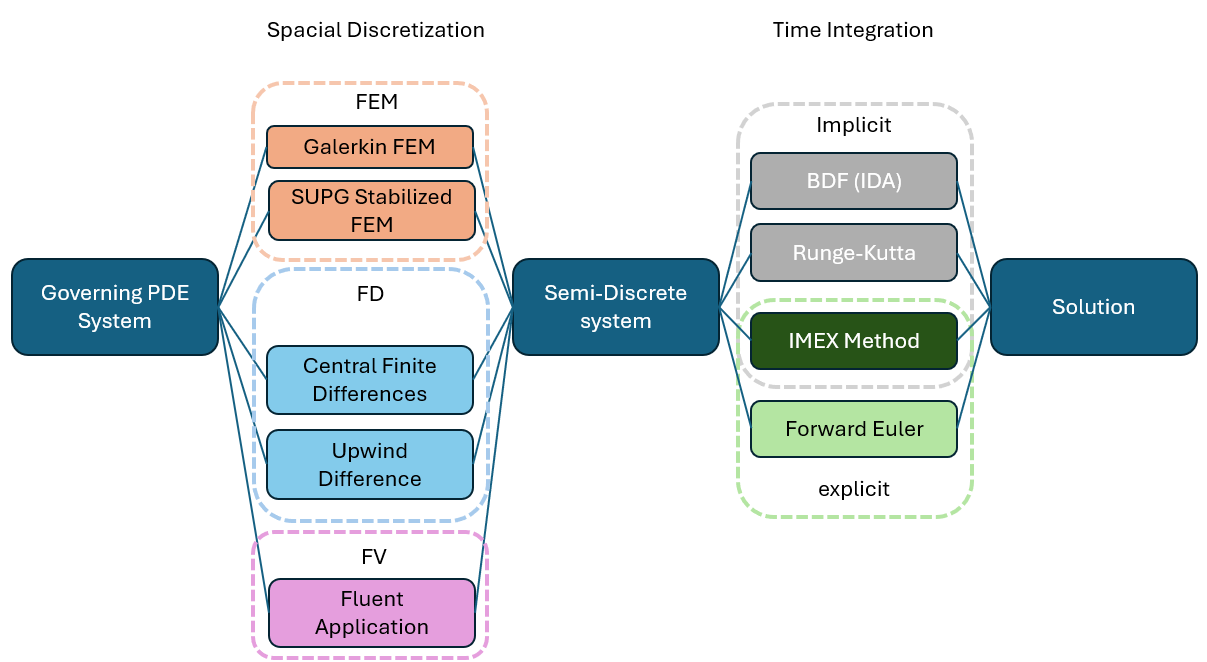
\includegraphics[width=\textwidth]{figures/Discretization_steps.png}
    \caption{The discretization steps to solve a PDE system. First we discretize in space, which we can do using Finite Differences, Finite Volumes, or Finite Elements. FD will be performed to check and validate solutions, and will be done using central finite differences, and Upwind methods. However this method quickly falls off and destabilizes for high Peclet numbers. We will create two types of FEM: the standard Galerkin method and the SUPG method for cases with a high Peclet number. Finite Volume is not looked at in this thesis, but is used in Darcy, and is very common in fluid models. Time integration is essentially independent from the spatial discretization, however often the best choice for time integration method is based on your choice of spatial discretization. These methods can be divided into Implicit and Explicit methods. We create our own IMEX method that combines both approaches. For our FEM with non-linear mass matrices, we will opt to use the IDA method, since we otherwise need to calculate an inverse or LU discretization at each time step. For a linear FEM with constant mass matrices, we use a fully implicit method. There are way more different discretization schemes, but these are the ones discussed in our thesis. It is also valuable to note that each spatial discretization is not unique; for example, you can often apply a Galerkin discretization on different spaces, giving different semi-discrete systems.}\label{fig:num_discretization_steps}
\end{figure}

